\documentclass[11pt]{article}
\usepackage[T1]{fontenc}
\usepackage[utf8]{inputenc}
\usepackage{lmodern,microtype,amsmath,amssymb,amsthm,mathtools}
\usepackage[a4paper,margin=28mm]{geometry}
\usepackage{xcolor,xurl,enumitem,booktabs,tikz}
\usetikzlibrary{arrows.meta,calc}
\usepackage[unicode,colorlinks=true,linkcolor=blue!45!black,
 citecolor=green!35!black,urlcolor=blue!55!black]{hyperref}
\setlength{\emergencystretch}{2em}
\numberwithin{equation}{section}
\newtheorem{theorem}{Theorem}[section]
\newtheorem{proposition}[theorem]{Proposition}
\newtheorem{lemma}[theorem]{Lemma}
\newtheorem{corollary}[theorem]{Corollary}
\theoremstyle{definition}\newtheorem{definition}[theorem]{Definition}
\theoremstyle{remark}\newtheorem{remark}[theorem]{Remark}
\title{Triangular insertion and volume limits for augmented diagrams}
\author{}\date{}
\begin{document}\maketitle
\begin{abstract}
A triangulated disk can replace a triangular face of a marked
augmented diagram without changing the coefficient demands on its
boundary. We prove an exact identity for the disk's minimized circle
potential, including the limit in which two boundary curvatures
vanish. This identity transports a finite shared-radius certificate
from a protected diagram to a sufficiently thin ordinary face.
Every fixed finite collection of certified blocks admits such an
insertion into an explicit family of cores. Separate finite-source,
asymptotic and geometric theorems then give the full volume limit for
independently long fixed signed fillings of the resulting knots.
An explicit sequence has a uniform source gap while failing complete
weak balance at its recorded mark. The argument preserves the
original shared face targets and proves neither a finite polynomial
star--triangle identity nor a uniform theorem for growing diagrams.
\end{abstract}

\section{Insertion and the volume theorem}

A marked diagram in this paper is encoded by a finite oriented simple
triangulated sphere and a perfect matching of its dual. Each matched
pair of triangles specifies a two-strand crossing circle. A chosen
nonmatching edge is the mark: its endpoints are assigned zero face
variables, and all other vertices are \emph{ordinary}. The inverse-cut
construction of \cite[Section 2 and Proposition 2.1]{Marked} realizes
these data as an augmented link in \(S^3\), with its crossing disks and
their primitive meridian--longitude bases retained. The final outside
strand connections must form one component whenever we call its
filled link a knot.

An ordinary triangular face has three positive coefficient weights. It need not contain either protected face of the marked source. This paper proves that a diagram already controlled at a protected edge can be inserted at such an ordinary face when two boundary curvatures are sufficiently small relative to the third. The coefficient demands on the old boundary vertices remain the original core demands.

The mechanism has two parts. The complete packing inside a triangular boundary contributes exactly the old triangle potential plus a constant. For complementary sectors, the old protected certificate extends to small positive boundary weights. Any local comparison error is absorbed by the same boundary correction. Explicit strictly balanced cores supply arbitrarily thin ordinary faces, so the theorem applies to any fixed finite collection of certified inputs.

\begin{theorem}[Ordinary triangular insertion]\label{ti:main} Let \(B_1,\ldots,B_s\), \(s\ge1\), be fixed marked simple-sphere diagrams satisfying the unabridged certificate \eqref{ti:eq-C2}. Choose a marked boundary triangle in each input. There are positive boundary thresholds \(\eta_j\) such that the following holds.

Let \(D\) be a fixed certified core, with chosen witnesses for every locally allowed noncentral string and its complete vector. Select \(s\) distinct matching pairs and one all-ordinary triangle in each, with no pair used twice. At the \(j\)-th triangle, write its weights as \((u_j,v_j,b_j)\). Suppose every chosen core vector satisfies
\begin{equation}\label{ti:eq-T1}
u_j/b_j\le\eta_j,\qquad v_j/b_j\le\eta_j.
\end{equation}
Insert the rooted disks of the \(B_j\)'s by the oriented operation in Section~\ref{ti:sec-5}. The resulting marked simple sphere has an unabridged full-source certificate with gap at least
\begin{equation}\label{ti:eq-T2}
\min\{\gamma_D,\gamma_{B_1}/2,\ldots,\gamma_{B_s}/2\}.
\end{equation}
Its complete action is \(\Phi_D+\sum_j\Phi_{B_j}\).

Such cores exist explicitly for every fixed finite list of inputs: the even zigzag chains of Section~\ref{ti:sec-8} have terminal boundary ratios tending to zero, and their complete vector is a witness for every noncentral string. Choose any retained half-twist pattern whose final strand connections form one knot. All independently sufficiently long fixed signed primitive fillings of the final crossing circles satisfy the full volume limit \eqref{ti:eq-27}, at both parities and composite levels.

The construction may change knot type. The filling threshold depends on the entire fixed assembled diagram and its retained pattern. No growing-diagram or level-dependent-twist limit is asserted.
\end{theorem}

\section{The original source and the disk action}\label{ti:sec-1}

An input is a finite simple oriented triangulated white sphere with at least four vertices, a perfect matching of its dual triangles, and a marked nonmatching edge. The literal inverse cut of \cite[Section 2]{Marked} supplies its augmented link in \(S^3\), with the cyclic crossing orders and the original twice-punctured crossing disks retained. A matched pair is one crossing-circle region. The two endpoints of the mark are the protected zero variables; every other white vertex has coefficient target \(d=N-1\). There are \(R\) ordinary vertices and \(R\) matched pairs.

For clarity, the finite source behind the certificate is fixed here.
At level \(N\ge3\), set \(d=N-1\), \(J=\lfloor d/2\rfloor\),
\(\theta=\pi/N\), and \(s_j=2\sin(j\theta)\). On
\(1,z,\ldots,z^d\), use the polynomial operator
\begin{equation}\label{ti:operator}
\mathsf C z^j=2\cos((2j+1)\theta)z^j
-s_j^2(x+y)z^{j-1}-s_js_{j-1}xy z^{j-2},
\end{equation}
with absent terms zero. If \(T_N\) is the Chebyshev polynomial and
\(\chi_N(t)=2T_N(t/2)+2\), define the polynomial divided difference
\[
V_N(\sigma;\mathsf C)=
\frac{\chi_N(\sigma)-\chi_N(\mathsf C)}{\sigma-\mathsf C},\qquad
H_V(x,b,c,y;\sigma)=\sum_{0\le i\le j\le d}
       V_N(\sigma;\mathsf C)_{ij}b^ic^{d-j}.
\]
Here the quotient denotes a polynomial identity, not an inverse at
an eigenvalue. The three disjoint row selections are
\[
C:\ i\le J,\ d-j\le J;\qquad
L:\ d-j>J;\qquad R:\ i>J.
\]
They exhaust the entries since \(i\le j\). At a protected overload
the corresponding homogeneous monomials vanish. With the same face
variable at every occurrence, the original shared source is
\begin{equation}\label{ti:finite-source}
S_{D,N}(\boldsymbol\sigma)=
\left[\prod_{f\in\mathcal O_D} L_f^d\right]
\left.\prod_e H_V(L_{x_e},L_{b_e},L_{c_e},L_{y_e};\sigma_e)
\right|_{L_u=L_v=0}.
\end{equation}
It has separate spectral degree at most \(d\). Write \(C_{D,N}\)
for its all-central selection. The exact identification with the
diagram, including its normalization, is an imported finite theorem
specified below; the insertion proof will retain exactly these targets.

For a nonnegative curvature vector \(w\), with at least one positive weight in each triangle, put
\begin{equation}\label{ti:eq-1}
\begin{aligned}
Q(w_1,w_2,w_3)&=
\max_{\substack{\alpha_i\ge0\\\alpha_1+\alpha_2+\alpha_3=1/2}}
\left\{\sum_i f(\alpha_i)+\sum_{w_i>0}\alpha_i\log w_i\right\},\\
f(t)&=\frac{\Lambda(\pi t)+\Lambda(\pi/2-\pi t)}{\pi}.
\end{aligned}
\end{equation}
where loads at a zero weight are required to vanish and
\(\Lambda(s)=-\int_0^s\log(2\sin r)\,dr\). In particular \(f(0)=f(1/2)=0\), \(f\ge0\), and \(f\) is strictly concave on \((0,1/2)\).

For an ordered polynomial quartet \((x,b,c,y)\), the input and output triangles are \((x,b,y)\) and \((x,c,y)\). The complete and one-sided rate functions are
\begin{equation}\label{ti:eq-C1}
\begin{aligned}
X&=Q(x,b,y)+Q(x,c,y),\\
A_L&=\max\{\log c,Q(x,b,y)+\tfrac12\log c\},\\
A_R&=\max\{\log b,Q(x,c,y)+\tfrac12\log b\}.
\end{aligned}
\end{equation}
The label \(L\) overloads the middle \(c\), and \(R\) overloads \(b\). A label overloaded at a protected zero is absent from the finite source. These are the phase-uniform bounds on the whole real spectral interval
of \cite[Theorem 1.1]{Local}. Both level parities and the unused
recurrence factors in the original source are included. The label
\(C\), written \(\mathrm C\) in the companion papers, means central.

For a whole string \(\omega\) of locally allowed labels \(C,L,R\), put \(A_{e,C}=X_e\), \(q_f=\log w_f\), and
\begin{equation}\label{ti:eq-C2a}
G_{D,\omega}(q)=\sum_e A_{e,\omega_e}(q)-\sum_{f\in\mathcal O_D}q_f,
\qquad P_D=G_{D,C},\qquad
\Phi_D=\min P_D=\frac{\operatorname{Vol}(Y_D)}{2\pi}.
\end{equation}
Here \(Y_D\) is the original augmented exterior before crossing-circle filling.
\begin{definition}[Unabridged certificate]\label{ti:certificate}
This is the certificate of \cite[Definition 3.1]{Planar}. A finite unabridged certificate means that there is \(\gamma_D>0\) and, for every locally allowed \(\omega\ne C\), a real log-weight vector \(q^\omega\) with
\begin{equation}\label{ti:eq-C2}
G_{D,\omega}(q^\omega)\le\Phi_D-\gamma_D.
\end{equation}
The same face weight is used at every occurrence within a string. Different strings may use different witnesses. Strings whose global coefficient happens to vanish are still included. Only local protected-overload zeros are omitted. There are finitely many strings because the diagram is fixed.
\end{definition}
Every local rate has logarithmic homogeneity one. Since the number
of ordinary targets equals the number of regions, \(G_{D,\omega}\)
is invariant under scaling all ordinary weights by the same positive
constant. We may therefore normalize any chosen ordinary weight to one.

Weak balance means \(X_e\ge\log b_e,\log c_e\) at the complete
packing, omitting a comparison whose middle weight is zero. It supplies
an unabridged certificate by \cite[Theorem~4.3]{Planar}; the
forty-branch seventeen-region example of \cite[Theorem~6.1]{Planar}
supplies another. The input hypothesis is strictly about these actual rate functions and original demands. It does not assume the desired gap for an assembled diagram.


\begin{proposition}[The imported source and geometry interface]
\label{ti:imports}
For every fixed marked simple sphere as above, the following five
results apply to its original source and crossing disks.
\begin{enumerate}[label=\textup{(\roman*)},leftmargin=*]
\item The exact diagram theorem
\cite[Theorem 9.1 and Corollary 9.2]{Finite} identifies
\eqref{ti:finite-source} with the marked spectral evaluation.
For fixed signed powers \(n_e\), a polynomial functional
\(\mathcal L_N^{n_e}\) fills each box, and
\[
A_{\rm raw}(\boldsymbol n)=
 (\bigotimes_e\mathcal L_N^{n_e})S_{D,N},\qquad
\left| (\bigotimes_e\mathcal L_N^{n_e})F\right|
\le\prod_e(1+|n_e|/2)\|F\|_{[-2,2]^R}.
\]
The degree condition is \(\deg_{\sigma_e}F\le N-1\).
The norm is \cite[Theorem 1.1]{Finite}; it holds abstractly even at
\(N=2\), whereas the diagram application here is \(N\ge3\).
For a knot, \cite[Theorem 10.1]{Finite} gives
\(\langle K\rangle_N=\zeta_{N,D}A_{\rm raw}\) with
\(|\zeta_{N,D}|=1\). The reduced zero-framed invariant has unknot
value one, and its quantum parameters are
\(q_N=e^{\pi i/N}\), \(q_N^2=e^{2\pi i/N}\).
\item The local estimate \cite[Theorem 1.1]{Local} bounds every genuine
sector by \eqref{ti:eq-C1} on one shared torus, uniformly in its
phases and \(\sigma_e\in[-2,2]\). Its error is subexponential
for a fixed diagram and a fixed positive supported radius vector.
Consequently a witness \(G_{D,\omega}\le\Phi_D-\gamma\)
bounds that sector coefficient by
\(\exp\{N(\Phi_D-\gamma+o(1))\}\).
\item For the same simple sphere, the positive complete vector gives
the holomorphic central coefficient expansion and the strict outer
spectral-strip bound of \cite[Theorem 1.1]{Source}. In particular its
finite face-critical action \(A_N(\delta)\) converges with derivatives
to an even classical action \(A_0(\delta)\), with
\(A_0(0)=\Phi_D\) and negative definite spectral Hessian there.
The finite face Hessian and the leading coefficient are nonzero.
This statement concerns \(C_{D,N}\), not the complementary source.
\item Applied to those hypotheses,
\cite[Theorem 1.1]{Oscillatory} evaluates the entire original
central filling period for independently sufficiently long fixed
signed powers. If \(\delta_{N,\mathbf1}\) is the critical point of
\[
A_N(\delta)+\pi i\sum_e n_e\delta_e^2
                       +2\pi i\sum_e\delta_e,
\]
its value \(S_{N,\mathbf1}\) converges to \(S_{\boldsymbol n}\).
The remaining prefactor is nonzero and subexponential. Thus
\[
\lim_{N\to\infty}\frac1N\log
\left|(\bigotimes_e\mathcal L_N^{n_e})C_{D,N}\right|
=\operatorname{Re}S_{\boldsymbol n},\qquad
\operatorname{Re}S_{\boldsymbol n}\longrightarrow\Phi_D
\quad(\min_e|n_e|\to\infty).
\]
Both limits retain the original parity phases; no unsigned Fourier
replacement is made.
\item Independently of quantum asymptotics,
\cite[Proposition 2.1, Section 2.3 and Theorem 1.1]{Marked} constructs
the complete exterior \(Y_D\), gives
\(\operatorname{Vol}(Y_D)=2\pi\Phi_D\), and identifies the above
classical action with its primitive filling action. For
\(n_e=\epsilon_e-2p_e\), the selected solution satisfies
\(U_e+p_eV_e=-2\pi i\) in the original disk framing.
For independently long fixed powers it completes smoothly along
that primitive slope, keeps the main cusps complete, and satisfies
\(2\pi\operatorname{Re}S_{\boldsymbol n}
=\operatorname{Vol}(S^3\setminus K_{\boldsymbol n})\)
when the final strand pairing is a knot. This is an absolute
fundamental-chain comparison on the original filled manifold.
\end{enumerate}
\end{proposition}

These statements are the precise foundation results used below.
They do not supply a general complementary-source gap. That additional
inequality is what the certificate and its transport must prove.
The identification of the limiting triangle action in (iii) with the
classical one in (v) uses their displayed triangle derivative and their
common value \(\Phi_D\); it is part of those companion statements,
not a new normalization chosen here.

Let \(B\) be a simple triangulated oriented sphere with at least four vertices. Remove one face \(f=(u,b,v)\), leaving a triangular disk \(P\). Let \(I\) be its \(k\) interior vertices. The disk has \(2k+1\) triangles. The boundary-dependent disk action is
\begin{equation}\label{ti:eq-2}
J_{u,v,b}(q_I)=\sum_{t\subset P}Q_t(w)-\sum_{i\in I}q_i,
\qquad w_i=e^{q_i},\qquad
\mathcal J_P(u,v,b)=\inf_{q_I}J_{u,v,b}(q_I).
\end{equation}
Only interior targets are subtracted here. The three boundary loads
are free. Once the interior demands hold, their aggregate is \(1/2\):
the disk supplies \(k+1/2\) and its interior consumes \(k\). The claim is
\begin{equation}\label{ti:eq-3}
\boxed{\ \mathcal J_P(u,v,b)=Q(u,v,b)+C_P\ }\qquad(u,v,b>0).
\end{equation}
The constant is determined below. This is an identity of classical source actions with their absolute normalization.

\begin{theorem}[A disk with prescribed boundary curvatures]
\label{ti:disk}
Let \(P\) be obtained by removing a face from a finite simple
triangulated sphere. For every \(u,v,b>0\), the action
\eqref{ti:eq-2} has a unique finite minimizer. Its tangent circles
develop injectively into the triangular interstice determined by the
three boundary circles. If the boundary edge \(uv\) is the protected
mark of the original block, then
\[
 \mathcal J_P(u,v,b)=Q(u,v,b)+\Phi_B.
\]
With \(b>0\) fixed, the identity extends to \(u,v\ge0\). The
minimizers converge to the unique supported minimizer at \(u=v=0\).
No coefficient target is imposed on any boundary vertex in this
disk action.
\end{theorem}
Sections~\ref{ti:sec-2}--\ref{ti:sec-4} prove the theorem, including
existence at the two-zero boundary rather than only a formal
continuation of the positive equations.

For a triangle with positive supported weights, its unique maximizing loads are
\begin{equation}\label{ti:eq-4}
\alpha_i=\frac1\pi\arctan\frac{w_i}{D_t},
\qquad D_t=\sqrt{w_1w_2+w_2w_3+w_3w_1}.
\end{equation}
For two positive weights this is interpreted on those two corners; a singleton has load \(1/2\). The Hessian in supported log weights is a Laplacian, with off-diagonal entries
\begin{equation}\label{ti:eq-5}
-\kappa_{ij},\qquad
\kappa_{ij}=\frac{w_iw_j}{2\pi D_t(w_i+w_j)}>0.
\end{equation}
Singletons contribute no Hessian. Thus a connected supported graph has only the common-scale kernel.

These formulas follow directly from the potential, with no packing
existence assumption. Indeed \(f'(t)=\log\cot(\pi t)\), so the
Lagrange multiplier equations give
\(\tan(\pi\alpha_i)=w_i/D_t\); the sum of the angles is \(\pi/2\)
exactly when \(D_t^2=\sum_{i<j}w_iw_j\). Differentiating for
distinct \(i,j,k\), and using
\(D_t^2+w_i^2=(w_i+w_j)(w_i+w_k)\), gives
\eqref{ti:eq-5}. Homogeneity gives zero row sums. The associated
quadratic form is \(\sum_{i<j}\kappa_{ij}(h_i-h_j)^2\).

\section{Existence for every positive boundary triple}\label{ti:sec-2}

Here is the finite feasibility and coercivity argument, separate from the subsequent development.

Each triangle supplies \(1/2\); every interior vertex demands one. Pool the three boundary destinations into one destination of demand \(1/2\), retaining their separate corners. A strictly positive transport table exists.

For a nonempty set \(S\) of interior destinations, put \(T=I\setminus S\). Puncture the capped sphere at a vertex of \(S\). The triangles supported on \(T\cup\{u,v,b\}\) are bounded faces of a simple planar graph on \(|T|+3\) vertices. There are at most \(2|T|+1\) bounded triangular faces; one is the removed face. Thus at most \(2|T|\) disk triangles miss \(S\), so at least \(2|S|+1\) touch it. Their supply is strictly greater than \(|S|\).

A proper destination set containing the boundary pool has nonempty complement \(T\subset I\). Triangles wholly on \(T\) number at most \(2|T|-5\) for \(|T|\ge3\), and none for \(|T|\le2\). The touching supply therefore strictly exceeds that set's demand. The full destination set has equality of totals. These are the strict finite transport Hall inequalities. For
completeness, the finite supply--demand criterion follows by augmenting
along alternating paths in the bipartite incidence graph: if the
required total flow has not been reached and no augmenting path remains,
the destinations reachable from an unsatisfied destination give a set
whose demand exceeds its adjacent supply. Conversely such a set
precludes a feasible flow. Thus the displayed inequalities give a
feasible table. Subtracting one sufficiently small positive amount from every allowed corner preserves feasibility; restoring those amounts gives a table \(\alpha^0_{ti}>0\) on every corner.

Fix positive boundary weights. For an interior direction \(h\), extend \(h\) by zero on the boundary. The recession of \eqref{ti:eq-2} is
\begin{equation}\label{ti:eq-6}
\mathcal R(h)=\frac12\sum_t\max_{i\in t}h_i-\sum_{i\in I}h_i
=\sum_t\sum_{i\in t}\alpha^0_{ti}
                  \left(\max_{j\in t}h_j-h_i\right).
\end{equation}
It is nonnegative. Equality forces \(h\) to be constant on every triangle. The disk graph is connected and the boundary is grounded, so equality forces \(h=0\). Compactness of the unit sphere gives a positive recession margin.

More explicitly, \(Q_t(q)\ge\frac12\max_{i\in t}q_i\), while its difference from that maximum is bounded above by the finite maximum of \(\sum f\). Fixed boundary logarithms alter these estimates only by a bounded constant. Consequently
\begin{equation}\label{ti:eq-7}
J_{u,v,b}(q_I)\ge c\lVert q_I\rVert-C.
\end{equation}
for constants \(c>0,C<\infty\). This proves coercivity, not merely strict convexity. The grounded Hessian \eqref{ti:eq-5} is positive definite, so the minimizer exists, is finite, and is unique. Its loads satisfy each interior demand exactly.

The resulting minimizer depends smoothly on the positive boundary log weights by the implicit function theorem and the positive definite interior Hessian.

\section{Development and proof of the fixed-boundary identity}\label{ti:sec-3}

Set radii \(r_i=1/w_i\). For each triangle, the three lengths \(r_i+r_j\) form a nondegenerate triangle. Its center angle at \(i\) is \(2\pi\alpha_{ti}\), by the tangent-circle half-angle formula \eqref{ti:eq-4}.
Explicitly, the usual half-angle identity for a triangle gives
\[
\tan\frac{\Theta_i}{2}
=\sqrt{\frac{r_jr_k}{r_i(r_i+r_j+r_k)}}
=\frac{w_i}{\sqrt{w_iw_j+w_iw_k+w_jw_k}},
\]
which fixes both the factor \(2\pi\) and the curvature convention.

At the minimizer every interior vertex has total angle \(2\pi\). All boundary corner angles are positive; their sum over the three boundary vertices is \(\pi\), because there are \(2k+1\) triangles and \(k\) interior vertices. In particular every boundary angle sum is less than \(\pi\).

Develop the triangles with their given orientation. Continuation around an interior vertex has rotation \(2\pi\) and zero translation. Such loops generate the holonomy of the punctured disk, so the development is single-valued. Its boundary consists of three straight segments of lengths \(r_u+r_v,r_v+r_b,r_b+r_u\), traversing the prescribed convex center triangle once.

This development is injective. For a point outside the finite developed edges, each preimage is orientation preserving, so the number of preimages equals the boundary winding number: one inside the boundary triangle and zero outside. Local injectivity at edges and interior vertices, followed by continuity, extends this to the whole disk. Separating triangles inside \(P\) cause no change in this degree argument.

It follows that the total developed angle \(\Theta_u\) at the boundary vertex \(u\) is exactly the angle of the unrefined center triangle. Differentiating the optimized action gives
\begin{equation}\label{ti:eq-8}
\partial_{\log u}\mathcal J_P
=\frac{\Theta_u}{2\pi}
=\frac1\pi\arctan\frac{u}{\sqrt{uv+ub+vb}}
=\partial_{\log u}Q(u,v,b).
\end{equation}
The same holds at \(v,b\). Hence the difference in \eqref{ti:eq-3} has zero differential throughout the connected positive octant and is constant. There is no extra boundary-linear term. Its logarithmic homogeneity is \(1/2\), since the disk has half-supply \(k+1/2\) and interior demand \(k\).

The developed disks have disjoint interiors and only the prescribed contacts: each disk sector lies inside its incident center triangle and stops before the opposite center edge. This identifies the variational development with the circle packing
in the bounded triangular interstice. When the disk is inserted into
the closed simple sphere, the contact-circle halfspaces and their
original pairings are those of \cite[Proposition 2.1]{Marked}; that
result supplies the convex ideal pieces and the augmented exterior.
The flat development alone is not being used as a volume formula.

\section{Two zero boundary weights: coercivity, uniqueness and the limit}\label{ti:sec-4}

Now take \(u=v=0,b=1\). Every triangle of \(B\) has an ordinary supported corner. Write \(O=I\cup\{b\}\). On the full sphere assign demand one to every member of \(O\), and supply \(1/2\) to each triangle.

This supported transport has a strictly positive table on every allowed corner. For a nonempty proper \(S\subset O\), put \(T=O\setminus S\). Puncture at a vertex of \(S\). Triangles missing \(S\) are bounded triangular faces of a simple planar graph on \(|T|+2\) vertices, at most \(2|T|-1\). Thus at least \(2|S|+1\) sphere triangles touch \(S\). The full destination set has equality of totals. Subtracting a small positive corner amount yields strict relative feasibility, with singleton rows fixed at their forced \(1/2\) load.

The removed face \((u,b,v)\) is such a singleton. Removing its load leaves interior demands one and \(b\)-demand \(1/2\) in the disk. Let \(\alpha^0\) be the resulting strictly supported table.

Deleting \(u,v\) from a simple triangulated sphere leaves a connected graph. One direct proof deletes \(u\) by rerouting a path through its cyclic link, then deletes \(v\) by rerouting through its link with \(u\) removed, which is still connected. Removing the face \((u,b,v)\) removes no edge between two ordinary vertices. Therefore the supported co-occurrence graph of the disk is connected to \(b\).

For \(h_b=0\), the same formula as \eqref{ti:eq-6}, now using only supported corners, gives
\begin{equation}\label{ti:eq-9}
\mathcal R_0(h)=
\sum_t\sum_{i\in\operatorname{supp}(t)}
\alpha^0_{ti}\left(\max_{j\in\operatorname{supp}(t)}h_j-h_i\right)>0
\quad(h\ne0).
\end{equation}
It proves \(J_{0,0,1}(q)\ge c_0\lVert q\rVert\) up to a harmless constant. Formula \eqref{ti:eq-5} grounds the only kernel. There is consequently a unique finite minimizer \(q^0\).

The full protected-sphere action is exactly \(J_{0,0,1}\): restoring the removed singleton contributes \(\frac12\log b\), and subtracting its ordinary target contributes \(-\log b\), both zero at \(b=1\). Hence
\begin{equation}\label{ti:eq-10}
\min J_{0,0,1}=\Phi_B.
\end{equation}
The simple-sphere calibration \cite[Section 2.3]{Marked} identifies \(2\pi\Phi_B\) with the augmented volume of \(B\). No full-source estimate is needed for \eqref{ti:eq-10}.

For \(u,v\ge0\), monotonicity of \(Q\) gives \(J_{u,v,1}\ge J_{0,0,1}\). Its interior Hessian retains that same connected positive support and it remains coercive; no Loewner comparison of the old and new Hessians is required. Its unique minimizer \(q^{u,v}\) satisfies
\begin{equation}\label{ti:eq-11}
J_{0,0,1}(q^{u,v})
\le J_{u,v,1}(q^{u,v})
\le J_{u,v,1}(q^0)\longrightarrow J_{0,0,1}(q^0).
\end{equation}
Here \(Q\) is continuous as supported weights tend to zero: maximizing loads at the disappearing corners tend to zero, their entropy tends to zero, and their logarithmic terms are nonpositive; the reverse inequality comes from the old supported maximizing load. Coercivity confines \(q^{u,v}\) to a compact set, and uniqueness implies
\begin{equation}\label{ti:eq-12}
q^{u,v}\longrightarrow q^0\qquad(u,v\to0).
\end{equation}
The convergence is joint and uniform on sufficiently small boundary squares: the upper bound in \eqref{ti:eq-11} is at most \(J_{\eta,\eta,1}(q^0)\) when \(u,v\le\eta\).

Taking this limit in \eqref{ti:eq-3}, with \(Q(u,v,1)\to0\), identifies its constant:
\begin{equation}\label{ti:eq-13}
C_P=\Phi_B.
\end{equation}
Equations \eqref{ti:eq-3} and \eqref{ti:eq-13} extend to the closed boundary square with \(b>0\) by the same monotonicity argument. In particular, for the closed expression with no \(u,v\) targets,
\begin{equation}\label{ti:eq-14}
\widehat P_B=\sum_{t\subset B}Q_t-\sum_{i\in I}q_i-\log b,
\qquad
\inf\widehat P_B=\Phi_B+\Delta,\quad
\Delta=2Q(u,v,b)-\log b\ge0.
\end{equation}
For a one-sided zero limit, keep \(u\ge0\) finite and let \(v\downarrow0\).
The common lower bound \(J_{0,0,1}\) confines the minimizers to a
compact set, while evaluation at any fixed finite interior vector
passes to the limit. The supported Hessian still contains the
connected graph grounded at \(b\). Thus existence, uniqueness and
the action identity hold on these boundary edges as well. This
argument does not assign a coefficient demand to the disappearing
boundary variable.
For positive boundaries, every interior packing disk has curvature at least
\begin{equation}\label{ti:eq-14a}
u+v+b+2\sqrt{uv+ub+vb}>\max(u,v,b).
\end{equation}
Indeed, let the three boundary centers and radii be \(p_i,r_i\). On their center triangle maximize \(r(z)=\min_i(|z-p_i|-r_i)\). It is nonpositive on the boundary, whose sides are covered by the two incident tangent disks, and positive in the interstice. At a positive interior maximum there cannot be just one active distance. With two active distances, their gradients either admit a common increasing direction, or are opposite; in the latter case the center lies between tangent boundary centers and the common empty radius is nonpositive. Thus all three distances are active. Eliminating the center from the three tangency equations gives \((k-u-v-b)^2=4(uv+ub+vb)\). At equal boundary curvatures the bounded-interstice disk takes the plus sign. The maximum empty radius varies continuously with the three positive boundary radii (maximize the continuous distance function on their continuously varying compact center triangle), and the two algebraic roots never meet on the positive octant. The plus sign therefore holds throughout that connected octant, proving \eqref{ti:eq-14a}. Every interior packing disk is contained in this interstice, so its radius cannot exceed that maximum. In particular the central conditional root always has \(a>v\) for positive boundary data.

The root middle \(a\in I\) has \(e^{q_a^{u,v}}\to e^{q_a^0}>0\). Thus \(a\ge v\) for all sufficiently small \(u/b,v/b\), after common scaling.

An equivalent boundary-load statement is available. Maximizing entropy subject to the interior demands and a boundary vector \(\beta\) of total \(1/2\) gives a closed concave function. Its conjugate is \eqref{ti:eq-3}. Closed concave duality therefore identifies that function with \(\sum f(\beta_i)+\Phi_B\) on the whole closed half-simplex. This preserves aggregate boundary loads, including zero loads; it does not add boundary coefficient demands.

\section{Oriented sewing and exact target allocation}\label{ti:sec-5}

Let the fixed core have its own protected nonmatching edge, away from the selected all-ordinary faces. At one selected core region and one block root use the polynomial argument orders
\begin{equation}\label{ti:eq-15}
e_D=(u,v,c,b),\quad f_D=(u,v,b);
\qquad
e_B=(u,a,v,b),\quad f_B=(u,b,v).
\end{equation}
The removed triangles have opposite orientations. Their common matching side is \(ub\), and their retained partners are \((u,b,c)\) and \((u,a,b)\). After gluing, those partners form the new region
\begin{equation}\label{ti:eq-16}
e_{\mathrm{new}}=(u,a,c,b).
\end{equation}

\begin{figure}[htbp]
\centering
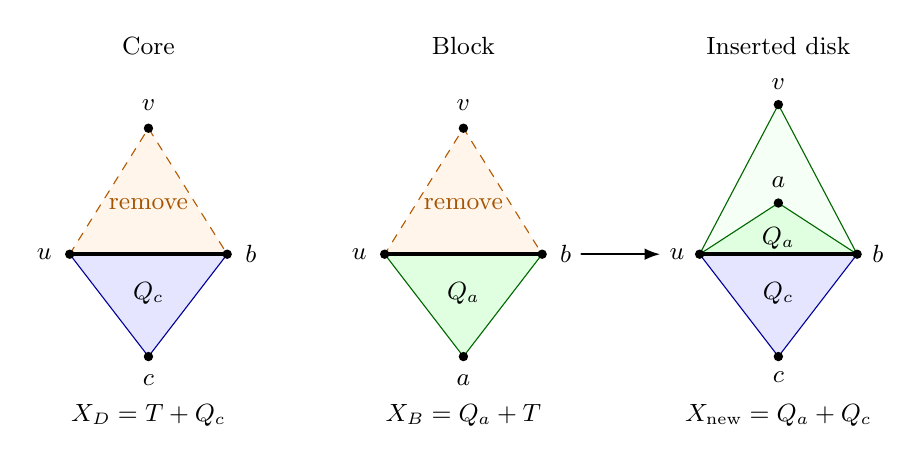
\begin{tikzpicture}[x=1cm,y=1cm,font=\small,
  line cap=round,line join=round,
  vertex/.style={circle,fill=black,inner sep=1.2pt},
  removed/.style={draw=orange!70!black,dashed,fill=orange!8},
  coreface/.style={draw=blue!60!black,fill=blue!10},
  blockface/.style={draw=green!40!black,fill=green!12}]
\begin{scope}
  \coordinate (u) at (0,0); \coordinate (b) at (2,0);
  \coordinate (v) at (1,1.6); \coordinate (c) at (1,-1.3);
  \path[removed] (u)--(v)--(b)--cycle;
  \path[coreface] (u)--(b)--(c)--cycle;
  \draw[line width=1.5pt] (u)--(b);
  \foreach \p/\where in {u/left,b/right,v/above,c/below}{
    \node[vertex] at (\p) {}; \node[\where=3pt] at (\p) {$\p$};
  }
  \node at (1,2.65) {Core};
  \node[orange!65!black] at (1,.63) {remove};
  \node at (1,-.5) {$Q_c$};
  \node at (1,-2.05) {$X_D=T+Q_c$};
\end{scope}
\begin{scope}[xshift=4cm]
  \coordinate (u) at (0,0); \coordinate (b) at (2,0);
  \coordinate (v) at (1,1.6); \coordinate (a) at (1,-1.3);
  \path[removed] (u)--(b)--(v)--cycle;
  \path[blockface] (u)--(a)--(b)--cycle;
  \draw[line width=1.5pt] (u)--(b);
  \foreach \p/\where in {u/left,b/right,v/above,a/below}{
    \node[vertex] at (\p) {}; \node[\where=3pt] at (\p) {$\p$};
  }
  \node at (1,2.65) {Block};
  \node[orange!65!black] at (1,.63) {remove};
  \node at (1,-.5) {$Q_a$};
  \node at (1,-2.05) {$X_B=Q_a+T$};
\end{scope}
\draw[-{Latex[length=2mm]},thick] (6.5,0)--(7.5,0);
\begin{scope}[xshift=8cm]
  \coordinate (u) at (0,0); \coordinate (b) at (2,0);
  \coordinate (v) at (1,1.9); \coordinate (a) at (1,.65);
  \coordinate (c) at (1,-1.3);
  \path[draw=green!40!black,fill=green!4] (u)--(v)--(b)--cycle;
  \path[blockface] (u)--(a)--(b)--cycle;
  \path[coreface] (u)--(b)--(c)--cycle;
  \draw[line width=1.5pt] (u)--(b);
  \foreach \p/\where in {u/left,b/right,v/above,a/above,c/below}{
    \node[vertex] at (\p) {}; \node[\where=2pt] at (\p) {$\p$};
  }
  \node at (1,2.65) {Inserted disk};
  \node at (1,.2) {$Q_a$};
  \node at (1,-.5) {$Q_c$};
  \node at (1,-2.05) {$X_{\rm new}=Q_a+Q_c$};
\end{scope}
\end{tikzpicture}

\caption{Insertion at an ordinary triangular face. The dashed faces are
identified with opposite orientations and removed; all three boundary
vertices remain. The thick side \(ub\) matches the two retained
triangles. In the inserted disk, the triangles above \((u,a,b)\) are
left unexpanded; the vertex \(v\) remains on their boundary.
Here \(T=Q(u,v,b)\), \(Q_a=Q(u,a,b)\), and \(Q_c=Q(u,c,b)\).
The old core supplies the sole targets at \(u,v\).
Only the \(b\)-target is duplicated in the comparison, giving
\(\Delta=2T-\log b\).}
\label{fig:triangular-boundary-insertion}
\end{figure}

Every other matching pair and cyclic order is retained. The four vertices of \eqref{ti:eq-16} are distinct because block interiors are fresh and \(a\) is an interior vertex.

Each boundary identification glues two punctured spheres along an embedded three-cycle. Fresh interiors give no loops or duplicate edges other than the boundary edges deliberately identified. The result is again a simple oriented triangulated sphere. The old common matching side is retained once and all other matching pairs are untouched. The core mark remains nonmatching.

If \(B\) has \(R_B=k+1\) regions, the insertion adds precisely \(k\) ordinary vertices and \(k\) matching regions. Its target count is
\begin{equation}\label{ti:eq-17}
\mathcal O_{\mathrm{new}}=\mathcal O_D\sqcup I,\qquad
R_{\mathrm{new}}=R_D+R_B-1.
\end{equation}
In particular, ordinary \(u,v\) retain their single core targets. They acquire no second targets from the block.

Put \(T=Q(u,v,b)\), \(Q_a=Q(u,a,b)\), \(Q_c=Q(u,c,b)\). Then
\begin{equation}\label{ti:eq-18}
X_D=T+Q_c,\quad X_B=Q_a+T,\quad X_{\mathrm{new}}=Q_a+Q_c.
\end{equation}
The block comparison expression subtracts its interior targets and one \(b\)-target, but none at \(u,v\). Combining it with the core therefore duplicates only \(b\). The exact complete action identity and a general sector inequality are
\begin{equation}\label{ti:eq-19}
P_{\mathrm{new}}=P_D+\widehat P_B-\Delta,\qquad
G_{\mathrm{new},\omega}\le
G_{D,\omega_D}+\widehat G_{B,\omega_B}-\Delta+\varepsilon_e,
\quad \Delta=2T-\log b.
\end{equation}
The local sector map is
\begin{equation}\label{ti:eq-20}
C\mapsto(C,C),\qquad L\mapsto(L,C),\qquad R\mapsto(C,R).
\end{equation}
Its defects may be taken to be
\begin{equation}\label{ti:eq-20a}
\varepsilon_C=0,\qquad
\varepsilon_L=(T-Q_a)_+,\qquad
\varepsilon_R=(T-Q_c)_+,\qquad
0\le\varepsilon_e\le\Delta/2.
\end{equation}
For example the old left expression after subtracting \(2T\) is
\(\max(q_c+Q_a-T,Q_a+q_c/2)\); adding \((T-Q_a)_+\) bounds the new left rate \(\max(q_c,Q_a+q_c/2)\). The right calculation interchanges \(a,c\). Finally \(Q_a,Q_c\ge\frac12\log b\), proving the last bound without any middle-order assumption.

Eliminating the block variables in the first equality of \eqref{ti:eq-19} using \eqref{ti:eq-14} gives, for every core vector, exactly \(P_D+\Phi_B\). Therefore
\begin{equation}\label{ti:eq-21}
\Phi_{\mathrm{new}}=\Phi_D+\Phi_B.
\end{equation}
All original core face derivatives and target demands are unchanged.

For finitely many attachments choose distinct core matching pairs; no removed face or its partner is used twice. Boundary vertices may coincide. Their weights remain the same core coordinates, and each retains one core target. Every block expression duplicates its own \(b\)-target once, and its own correction in \eqref{ti:eq-19} cancels that duplication, even when several such \(b\)'s are the same core vertex. Fresh interiors remain disjoint. Thus
\begin{equation}\label{ti:eq-22}
R_{\mathrm{new}}=R_D+\sum_j(R_{B_j}-1),
\qquad
\Phi_{\mathrm{new}}=\Phi_D+\sum_j\Phi_{B_j}.
\end{equation}

\section{From protected certificates to a full source estimate}\label{ti:sec-6}

Assume each block has a finite unabridged certificate at its standalone protected mark \(uv\), with gap \(\gamma_B>0\). It covers every locally allowed noncentral string, including old strings whose global extraction happened to vanish.

Choose one positive interior witness per old string at \(u=v=0,b=1\). Their rates are continuous when \(u,v\to0\), because every triangle contains a positive ordinary corner. Finiteness preserves half the gap on one common small square. A newly allowed side overloaded at \(u\) or \(v\) has rate
\[
\max\{\log u,\ Q_{\mathrm{retained}}+\tfrac12\log u\}
\]
or its \(v\)-analogue. At one fixed positive interior vector it tends uniformly to \(-\infty\); all other local factors are bounded above. This treats every newly allowed string. At an exactly zero overloaded weight the term is absent.

Combining these finite choices with \eqref{ti:eq-12}, there is \(\eta_B>0\) such that \(u/b,v/b\le\eta_B\) permits a central conditional minimizer of value \(\Phi_B+\Delta\), or a noncentral witness of value at most \(\Phi_B-\gamma_B/2\). The central conditional root satisfies \(a>v\) by \eqref{ti:eq-14a}; no ordering is required of noncentral witnesses.

Suppose the core has an unabridged certificate whose finitely many witnesses, together with its complete vector, meet the selected thin-boundary conditions. There is no required inequality between core middles. Choose one induced core witness, then classify each induced \textbf{whole block string}:

\begin{itemize}
\item
  If the entire block is central, use its conditional packing minimizer. Its root is central, so the new bridge can only be central or left. A central bridge is exact, and a left bridge has zero defect because \eqref{ti:eq-14a} gives \(a>v\) and hence \(Q_a\ge T\). Its value \(\Phi_B+\Delta\) cancels the \(-\Delta\) in \eqref{ti:eq-19}.
\item
  If the block has any noncentral label, use the finite extended certificate. Its value is at most \(\Phi_B-\gamma_B/2\), while its bridge defect is at most \(\Delta/2\). It therefore contributes at most \(\Phi_B-\gamma_B/2-\Delta/2\) after the correction.
\end{itemize}

The locally central root alone does not imply that the whole block is central. The split above uses every label of that block. At least one induced input is noncentral when the output is noncentral. For any fixed finite number of blocks this proves
\begin{equation}\label{ti:eq-23}
\gamma_{\mathrm{new}}\ge
\min\{\gamma_D,\gamma_{B_1}/2,\ldots,\gamma_{B_s}/2\}>0.
\end{equation}
All boundary incidences use the actual core weights. No summed defect budget is needed: each block absorbs its own defect.

The local bounds \eqref{ti:eq-C1} are uniform in phases and all real spectral variables at both parities. The number of sector strings is finite for the fixed assembly. Hence \eqref{ti:eq-23} bounds the entire complementary source polynomial on its original full real spectral cube. It is not an estimate for independent local radii or for a changed collection of face targets.

\section{Original primitive fillings and the actual volume conclusion}\label{ti:sec-7}

The new sphere and matching are fed into the original Morse inverse-cut construction. This constructs the augmented link \(Y_{\mathrm{new}}\) in \(S^3\), its crossing-circle balls, local signed half twists, outside strands and disk-framed primitive bases. It is not necessary to interpret the operation as a preexisting named topological sum.

There is one new crossing circle at each merged pair. Its primitive word is the ordered two-head product from its new quartet. The two input crossing circles do not survive as two independently fillable cusps. The independent integers in the conclusion belong to the \textbf{final} regions. Choose a retained parity pattern passing the final one-component test; such a pattern exists as follows. The underlying connected four-valent
strand graph has two allowed local pairings at each crossing box. Start
with any pairing. If its circuit decomposition has several components,
connectedness gives a box traversed by two distinct circuits. Switching
its pairing merges these two circuits. Repetition reduces the number
of circuits to one. The two choices are precisely the even and odd
box parities; the sign of a retained odd crossing can then be fixed. No old knot parity or knot type is silently transported.

The simple-sphere packing theorem \cite[Proposition 2.1]{Marked} applies to the final sphere and fixes its positive complete cells. Equations \eqref{ti:eq-21}--\eqref{ti:eq-22} identify its actual augmented action:
\begin{equation}\label{ti:eq-24}
2\pi\Phi_{\mathrm{new}}=\operatorname{Vol}(Y_{\mathrm{new}}).
\end{equation}
This is not a claim that filled volumes add.

The five companion results stated in Proposition~\ref{ti:imports} now apply to the final original Morse source. The exact scalar is retained; every final ordinary face has target \(d=N-1\), and each final spectral variable has degree at most \(d\). The full filling norm costs at most
\(\prod_e(1+|n_e|/2)\). The entire central period is nonzero at both parities for independently sufficiently long fixed signed powers.

The representation constructed from the final original circles has
\begin{equation}\label{ti:eq-25}
U_e+p_eV_e=-2\pi i,\qquad n_e=\epsilon_e-2p_e.
\end{equation}
The small individual-generator logarithms, nonunit auxiliary holonomy and primitive logarithmic period give smooth solid-torus completion. The main cusp remains complete. The original disk surgery is in \(S^3\), so the metric is on the final knot complement. The same boundary triangulation and relative fundamental chain supply the absolute regulator comparison
\begin{equation}\label{ti:eq-26}
2\pi\operatorname{Re}S_{\boldsymbol n}
=\operatorname{Vol}(S^3\setminus K_{\boldsymbol n}).
\end{equation}
No comparison manifold or only exponentiated filling equation is substituted.

Finally choose the fixed long-filling threshold so that
\(\Phi_{\mathrm{new}}-\operatorname{Re}S_{\boldsymbol n}
<\gamma_{\mathrm{new}}/2\). The full complementary contribution then has smaller exponential rate. For the original reduced, zero-framed invariant normalized by the unknot,
\begin{equation}\label{ti:eq-27}
\lim_{N\to\infty}\frac{2\pi}{N}
\log\left|\langle K_{\boldsymbol n}\rangle_N\right|
=\operatorname{Vol}(S^3\setminus K_{\boldsymbol n}).
\end{equation}
Every block, core length, retained parity and final integer is fixed first. The threshold may depend on the entire finite assembly; there is no claim uniform in growing assemblies or quantum-level-dependent powers.

\section{Explicit cores with arbitrarily thin ordinary faces}\label{ti:sec-8}

Start with the octahedral white sphere. Its poles are \(P,S\), its rim is \(v_0,v_1,v_2,v_3\), and the global protected mark is \(v_0v_1\). Orient the faces by
\begin{equation}\label{ti:eq-28a}
T_j=(P,v_{j+1},v_j),\qquad Z_j=(S,v_j,v_{j+1})
\quad(j\bmod4).
\end{equation}
Match \(T_0,T_1\), match \(Z_0,Z_1\), and match \(T_2,Z_2\) and \(T_3,Z_3\). The marked complete curvatures are
\begin{equation}\label{ti:eq-28b}
P=S=1,\qquad v_2=v_3=2,\qquad v_0=v_1=0.
\end{equation}
The original angle equations verify this directly. At a pole the loads are one singleton \(1/2\), two copies of \(\pi^{-1}\arctan(1/\sqrt2)\), and one copy of \(\pi^{-1}\arctan(1/(2\sqrt2))\); they sum to one. The ordinary rim equations follow from the complementary two-angle identities. Uniqueness of the marked complete solution then gives \eqref{ti:eq-28b}.

Put \(u=v_2,\ v=P,\ b_0=v_3,\ c=S\). The chosen all-ordinary face \(F_0=(u,v,b_0)\) is matched to \((u,b_0,c)\). Insert \(b_j\) into \(F_{j-1}\), replacing it by the three oriented triangles
\begin{equation}\label{ti:eq-28c}
F_j=(u,v,b_j),\qquad A_j=(u,b_j,b_{j-1}),\qquad
B_j=(v,b_{j-1},b_j).
\end{equation}
Each is a genuine stellar subdivision in the bounded interstice. The exterior disks do not move. The positive Soddy recurrence and its exact solution are
\begin{equation}\label{ti:eq-28}
\begin{aligned}
b_{j+1}&=b_j+3+2\sqrt{3b_j+2},\\
b_j&=3j^2+4\sqrt2\,j+2
   =3(j+\sqrt2)(j+\sqrt2/3),\qquad
\sqrt{3b_j+2}=3j+2\sqrt2.
\end{aligned}
\end{equation}

For any positive even \(n\), pair \(A_1\) with the old exterior partner, pair \(F_n,A_n\), and for \(1\le j<n\) pair \(B_j,B_{j+1}\) when \(j\) is odd and \(A_j,A_{j+1}\) when \(j\) is even. Every new triangle is used once.

\begin{figure}[htbp]
\centering
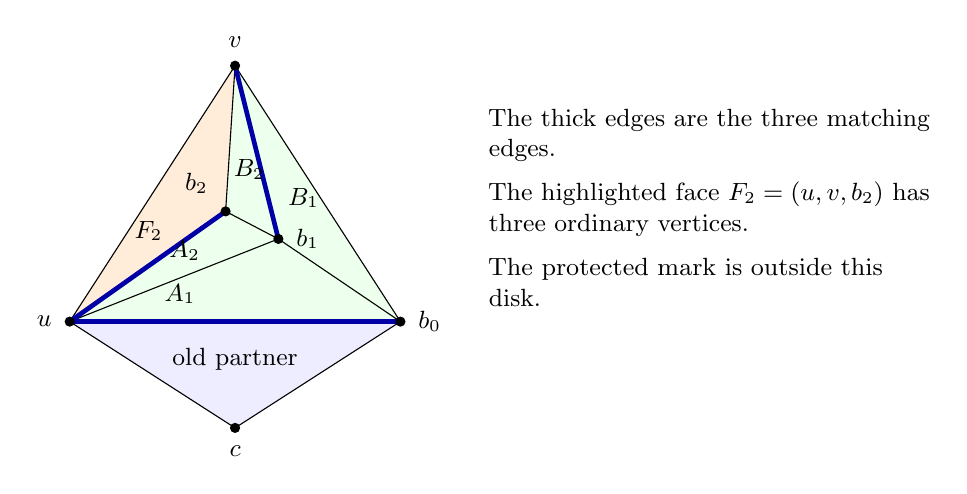
\begin{tikzpicture}[x=1cm,y=1cm,font=\small,
  line cap=round,line join=round,
  vertex/.style={circle,fill=black,inner sep=1.3pt}]
\coordinate (u) at (-2.1,0);
\coordinate (v) at (0,3.25);
\coordinate (b0) at (2.1,0);
\coordinate (b1) at (.55,1.05);
\coordinate (b2) at (-.12,1.40);
\coordinate (c) at (0,-1.35);
\fill[blue!7] (u)--(b0)--(c)--cycle;
\fill[green!7] (u)--(v)--(b0)--cycle;
\fill[orange!15] (u)--(v)--(b2)--cycle;
\draw (u)--(v)--(b0)--cycle;
\draw (u)--(b1)--(v) (b0)--(b1);
\draw (u)--(b2)--(v) (b1)--(b2);
\draw (u)--(c)--(b0);
\draw[line width=1.7pt,blue!65!black] (u)--(b0);
\draw[line width=1.7pt,blue!65!black] (v)--(b1);
\draw[line width=1.7pt,blue!65!black] (u)--(b2);
\foreach \p/\lab/\where in {u/u/left,v/v/above,b0/b_0/right,b1/b_1/right,b2/b_2/above left,c/c/below}{
  \node[vertex] at (\p) {}; \node[\where=3pt] at (\p) {$\lab$};
}
\node at (-1.1,1.15) {$F_2$};
\node at (-.70,.35) {$A_1$};
\node at (-.64,.90) {$A_2$};
\node at (.87,1.57) {$B_1$};
\node at (.18,1.93) {$B_2$};
\node at (0,-.48) {old partner};
\node[align=left,text width=5.6cm,anchor=west] at (3.1,1.45)
  {The thick edges are the three matching edges.\\[5pt]
   The highlighted face $F_2=(u,v,b_2)$ has three ordinary vertices.\\[5pt]
   The protected mark is outside this disk.};
\end{tikzpicture}

\caption{The ordinary-face construction with \(n=2\).
The pairs are \(A_1\) with the old partner across \(ub_0\),
\(B_1\) with \(B_2\) across \(vb_1\), and \(F_2\) with \(A_2\)
across \(ub_2\). All displayed vertices are ordinary.
For general even \(n\), successive subdivisions remain inside the
ordinary face and alternate the matching as stated in the proof.
The drawing records incidence and matching; the curvature values
are given by \eqref{ti:eq-28}.}
\label{fig:ordinary-triangular-zigzag}
\end{figure}
 The matching sides are \(ub_0\), \(ub_n\), and \(s_jb_j\), with \(s_j=v\) for odd \(j\) and \(s_j=u\) for even \(j\). They are the actual common edges with opposite face orientations in \eqref{ti:eq-28c}.

All these matching regions are strictly balanced. Here are the inequalities, including the finite constants. Write \(g=f(1/4)\), \(b_1=5+4\sqrt2\), \(b_2=14+8\sqrt2\). For each unchanged protected cap, the singleton at the pole and a quarter-quarter allocation at the pole and rim give
\begin{equation}\label{ti:eq-28d}
X-\log2\ge2g-\frac34\log2>\frac3{50}.
\end{equation}
The other unchanged region has outer weights \((2,0)\) and middle
weights \((1,1)\). Quarter loads on the two supported corners give
\(X\ge4g+\tfrac12\log2\). Thus its pure-middle and mixed-branch
differences are positive, with the quantitative margins below.

At the root region the outer weights are \(2,2\), the middles \(b_1,1\). Choose loads \((1/12,1/3,1/12)\) in the first triangle and \((1/5,1/10,1/5)\) in the second. Then
\begin{equation}\label{ti:eq-28e}
X-\log b_1\ge
2f(1/12)+f(1/3)+2f(1/5)+f(1/10)
+\frac{17}{30}\log2-\frac23\log b_1>\frac14.
\end{equation}
At each internal matched pair, put quarter loads at \(b_j,b_{j-1}\) in one triangle and at \(b_j,b_{j+1}\) in the other, with zero at \(s_j\). This gives
\begin{equation}\label{ti:eq-28f}
\begin{aligned}
X-\log b_{j+1}
&\ge4g-\frac14\log\frac{b_{j+1}^{\,3}}{b_j^2b_{j-1}}\\
&\ge4g-\frac14\log\frac{b_2^3}{2b_1^2}>\frac9{100}.
\end{aligned}
\end{equation}
The ratios \(b_j/b_{j-1}\) decrease by the factorization in \eqref{ti:eq-28}, and the expression in the first logarithm is \((b_{j+1}/b_j)^3(b_j/b_{j-1})\). This proves the second inequality for every \(j\), not just for bounded chain length.

The three strict constants can be checked with explicit interval arithmetic: use
\begin{equation}\label{ti:eq-28g}
\Lambda(x)=\frac12\sum_{r=1}^{K}\frac{\sin(2rx)}{r^2}
+E_K(x),\qquad |E_K(x)|\le\frac1{2K},\qquad K=2048.
\end{equation}
The resulting intervals for the three expressions are as follows.
\begin{center}
\begin{tabular}{@{}lc@{}}
\toprule
Expression & Certified containing interval\\
\midrule
\eqref{ti:eq-28d} & \((0.0629504,\,0.0635723)\)\\
\eqref{ti:eq-28e} & \((0.2543075,\,0.2561727)\)\\
\eqref{ti:eq-28f}, final lower bound & \((0.0985006,\,0.0997441)\)\\
\bottomrule
\end{tabular}
\end{center}
Only these fixed elementary constants use interval evaluation;
the all-length comparison is the exact ratio argument above.

At the final pair the outer weights are \(2,b_n\), and the middles \(1,b_{n-1}\). A vertex allocation at \(b_n\) and a quarter-quarter allocation at \(b_n,b_{n-1}\) give
\begin{equation}\label{ti:eq-28h}
X-\log b_{n-1}\ge2g+\frac34\log(b_n/b_{n-1})>0.
\end{equation}
This also bounds the smaller middle. The mixed-branch differences are bounded below by one of
\begin{equation}\label{ti:eq-28i}
2g-\frac14\log2,\quad
2g+\frac14\log(2/b_1),\quad
2g-\frac14\log(b_2/b_1),\quad
\frac12\log2,\quad 2g.
\end{equation}
Here is the assignment of these bounds to the actual matched pairs.
If \(h\) is the overloaded middle, its mixed difference is
\(Q(\hbox{outer}_1,h,\hbox{outer}_2)-\tfrac12\log h\).
Quarter loads at \(h\) and a positive outer weight \(w\) give
\(2g+\tfrac14\log(w/h)\); a vertex load at \(w\) gives
\(\tfrac12\log(w/h)\).
\begin{center}
\begin{tabular}{@{}lll@{}}
\toprule
Pair & Middle \(h\) & Lower bound for the mixed difference\\
\midrule
Protected cap & \(2\) & \(2g-\tfrac14\log2\)\\
Unchanged pair, outers \((2,0)\) & \(1\) & \(2g+\tfrac14\log2\)\\
Root, outers \((2,2)\) & \(b_1\) & \(2g+\tfrac14\log(2/b_1)\)\\
Root & \(1\) & \(\tfrac12\log2\)\\
Internal, outers \((s_j,b_j)\) & \(b_{j+1}\) &
 \(2g-\tfrac14\log(b_2/b_1)\)\\
Internal & \(b_{j-1}\) & \(2g\)\\
Tip, outers \((2,b_n)\) & \(b_{n-1}\) & \(2g\)\\
Tip & \(1\) & \(\tfrac12\log2\)\\
\bottomrule
\end{tabular}
\end{center}
The two internal cases use the decreasing ratios in
\eqref{ti:eq-28}; the tip uses \(b_n>b_{n-1}\).
All five bounds in \eqref{ti:eq-28i} exceed \(3/50\): use
\eqref{ti:eq-28d}, \(b_1<16\), \(b_2<8b_1\), and
\(\log2>1/2\).
Finally,
\[
 X-A_L=\min\{X-\log c,\ Q(x,c,y)-\tfrac12\log c\},
\]
and the analogous identity holds for \(A_R\).
The pure-middle bounds and this table therefore give a uniform
core certificate gap greater than \(3/50\) for every positive
even chain length. Its complete vector is the witness for every
noncentral string. Here \(n\) is the chain length; \(n_e\) denotes
a final signed crossing power.

The terminal ordinary face satisfies
\begin{equation}\label{ti:eq-29}
u/b_n=2/b_n\longrightarrow0,\qquad
v/b_n=1/b_n\longrightarrow0.
\end{equation}
Choose an even \(n\) large enough for the prescribed block threshold \(\eta_B\). This meets \eqref{ti:eq-T1} with the same complete vector for all core strings.

For finitely many inputs, first form a protected sum of finitely many octahedral cores, as in \cite[Theorem~5.3]{Planar}, leaving their \(T_2,Z_2\) pairs untouched. The complete vectors agree after the common joining weight is fixed.
The protected-gluing proof applies to these complete witnesses
themselves: its exact target correction and three local sector
comparisons retain their common positive gap. Thus a single complete
vector still witnesses every noncentral string. Build one chain in each selected disk. The old joined comparisons are unchanged, and \eqref{ti:eq-28d}--\eqref{ti:eq-28h} control every new region. Choosing the finite list of even chain lengths separately gives \eqref{ti:eq-T1} at every interface. Shared boundary vertices still carry the same core weight and one original target.

\subsection{Separation from protected sums and weak balance}\label{separation-from-protected-sums-and-weak-balance}

For one octahedral core, every subdivision and final block lies inside the all-ordinary disk \((v_2,P,v_3)\). The octahedron has no separating three-cycle. No new interior vertex is adjacent to either global protected vertex \(v_0,v_1\), so any three-cycle containing both protected vertices is unchanged and still bounds an original face.

Every nontrivial protected triangular sum at that mark creates a separating three-cycle containing the two protected vertices, with interior vertices on both sides. Therefore these one-core ordinary-face assemblies cannot be decomposed as a nontrivial protected sum at their recorded mark. This is a precise distinction of marked presentations, not a claim about all presentations of the resulting knot.

An explicit certified input also produces examples failing weak balance. Use the seventeen-region input of \cite[Theorem~6.1]{Planar} and attach at its crossing-15 face. Its restricted anchor-12 dual \cite[Equation (6.3)]{Planar} has zero loads at the protected vertices and mixes spectator rows only at \(2,4,7\). After assigning positive boundary weights the same rational table remains feasible, because it still assigns zero load to those two boundary variables. With \(b=1\), it gives
\begin{equation}\label{ti:eq-30}
\widehat G_{\mathrm{restricted}}(u,v;q_I)>
\Phi_B+\frac1{40}
\quad\text{for every positive interior vector}.
\end{equation}
If all four candidate regions \(2,4,7,12\) were weak-balanced at the conditional complete vector, their mixed spectators would equal their complete rates and the anchor would be at most its complete rate. Thus
\begin{equation}\label{ti:eq-31}
\widehat G_{\mathrm{restricted}}\le
\widehat P_B=\Phi_B+\Delta.
\end{equation}
Consequently \(\Delta<1/40\) forces at least one failure, and crossing 15 leaves all four candidates unchanged.

There is an elementary bound on this geometric correction. For \(A=u+v,\ P=uv\),
\begin{equation}\label{ti:eq-32}
\frac{d}{dt}Q(tu,tv,1)
=\frac{\arctan\sqrt{tA+t^2P}}{\pi t}
\le\frac{\sqrt A}{\pi\sqrt t}+\frac{\sqrt P}{\pi}.
\end{equation}
Integrating from zero gives
\begin{equation}\label{ti:eq-33}
\Delta=2Q(u,v,1)\le\frac4\pi\sqrt{u+v}+
\frac2\pi\sqrt{uv}.
\end{equation}
At the boundary in \eqref{ti:eq-29}, since \(b_n\ge3n^2\), \(\pi>3\) and \(2\sqrt2<\pi\),
\begin{equation}\label{ti:eq-34}
\Delta\le\frac4\pi\sqrt{\frac3{b_n}}
+\frac{2\sqrt2}{\pi b_n}
\le\frac4{3n}+\frac1{3n^2}<\frac1{40}
\qquad(n\ge64).
\end{equation}
This is a threshold for persistence of the balance failure only. The certificate extension may require a larger even \(n\), as determined by its finite witnesses. Taking both requirements gives arbitrarily large marked diagrams with the full invariant volume limit and a complete-packing balance failure.

\subsection{A fully specified infinite sequence}\label{a-fully-specified-infinite-sequence}

The original seventeen-region certificate gives a concrete threshold, with no search over knot invariants. Normalize each of its forty old witnesses at face 17. At chain length
\begin{equation}\label{ti:eq-35}
n_0=2^{20},\qquad
w_{16}=2/b_{n_0},\quad w_0=1/b_{n_0},\quad w_{17}=1,
\end{equation}
retain their other ordinary weights. Outward interval evaluation of the original rates proves a gap greater than \(1/50\) for all forty branches. The only newly allowed overloads are
\begin{equation}\label{ti:eq-36}
(0,R,0),\ (1,R,0),\ (12,L,16),\ (15,L,0),\ (16,L,0),
\end{equation}
where each triple lists the region, side, and overloaded face. For each, take that anchored side and all genuine spectator labels at one fixed old witness. The same evaluation gives a gap greater than \(1/50\) for these five branches. The forty old branches and five new anchors cover every locally allowed noncentral string, including any previously globally zero string.

The portable runner \href{https://github.com/sashakolpakov/murakamis_dream/blob/main/repro/check_triangular_boundary_certificate.py}{check\_triangular\_boundary\_certificate.py} checks the original Morse incidence and forty-branch division, the rational complete-flow demands, the five new anchors, and all forty-five rate inequalities with the Fourier tail in \eqref{ti:eq-28g}. It also replays the restricted dual used in \eqref{ti:eq-30}. These finite interval inequalities concern the source weights; they do not replace the all-length geometric or asymptotic proof.

Every selected rate is nondecreasing in \(w_0,w_{16}\), and the block comparison subtracts no target at these boundary vertices. Since \(b_n\) increases, the same forty-five witnesses work for every even \(n\ge n_0\). The correction \(\Delta\) also decreases. Combining their gap with the core gap \(>3/50\) and the whole-block comparison gives an assembled source gap at least \(1/50\).

\begin{corollary}[Explicit ordinary-face sequence]\label{ti:explicit} For every even \(n\ge2^{20}\), attach the seventeen-region block at crossing 15 to the terminal face of the length-\(n\) octahedral chain. The resulting original marked sphere has \(n+20\) regions, an unabridged full-source gap of at least \(1/50\), and a complete weak-balance failure among the retained regions \(2,4,7,12\). It has no separating three-cycle containing both protected endpoints. After choosing any final knot-producing parity, independently sufficiently long fixed signed primitive fillings satisfy \eqref{ti:eq-27}. Any fixed finite number of these blocks can similarly be attached to the multi-core construction, with the same source-gap lower bound. The filling threshold still depends on the entire fixed final diagram.
\end{corollary}

\section{Dependencies and finite certificate data}\label{ti:sec-9}

Variational approaches to Euclidean surface structures and circle patterns were developed by Rivin~\cite{Rivin1994} and Bobenko and Springborn~\cite{BobenkoSpringborn2004}. The argument above proves the required fixed-boundary existence and uniqueness directly, and fixes the disk action in the normalization of the original source. The source-certificate transport uses that explicit identity and the retained coefficient demands.

The complete disk identity is classical variational elimination with the original triangle normalization. It gives neither an equality of finite spectral polynomials nor an independent-radius source bound. The complementary estimates here use the actual phase-uniform rates \eqref{ti:eq-C1}, a shared torus for each string, and every original coefficient target.

The imported results are precisely those listed in
Proposition~\ref{ti:imports}, together with the protected certificate
definition, examples and gluing theorem of \cite{Planar}. The full
complementary estimate \eqref{ti:eq-23} is proved here. No open general
matched-sphere source estimate is used.

The explicit data are the original
\href{https://github.com/sashakolpakov/murakamis_dream/blob/main/experiments/actual_sector_cover_certificate.json}{seventeen-region cover}
and its
\href{https://github.com/sashakolpakov/murakamis_dream/blob/main/experiments/actual_shared_radius_anchor_obstruction_certificate.json}{restricted anchor certificate}.
The runner named above verifies their exact incidence and rational
demands before evaluating interval bounds. Its recorded output is
\href{https://github.com/sashakolpakov/murakamis_dream/blob/main/repro/triangular-boundary-insertion/summary.json}{the triangular-insertion summary}.
The checks of small oriented chains supplement the explicit all-length
construction \eqref{ti:eq-28c}; they do not prove that construction by
sampling. No knot invariant is evaluated by this certificate runner.

\begin{thebibliography}{9}
\bibitem{Finite}
\emph{Finite spectral evaluation and uniform filling bounds}.
\url{https://sashakolpakov.github.io/murakamis_dream/papers/filling-bounds.pdf}.
\bibitem{Local}
\emph{Uniform spectral bounds for local Casimir sources}.
\url{https://sashakolpakov.github.io/murakamis_dream/papers/local-coefficients.pdf}.
\bibitem{Source}
\emph{Holomorphic asymptotics of central shared face coefficients}.
\url{https://sashakolpakov.github.io/murakamis_dream/papers/source-asymptotics.pdf}.
\bibitem{Oscillatory}
\emph{Oscillatory filling sums with independently long twists}.
\url{https://sashakolpakov.github.io/murakamis_dream/papers/oscillatory-fillings.pdf}.
\bibitem{Marked}
\emph{Circle patterns and primitive fillings of augmented links}.
\url{https://sashakolpakov.github.io/murakamis_dream/papers/marked-fillings.pdf}.
\bibitem{Planar}
\emph{Shared face estimates and triangular gluing for planar link diagrams}.
\url{https://sashakolpakov.github.io/murakamis_dream/papers/planar-certificates.pdf}.
\bibitem{Rivin1994}
I. Rivin, Euclidean structures on simplicial surfaces and hyperbolic
volume, \emph{Ann. of Math.} \textbf{139} (1994), 553--580.
\url{https://doi.org/10.2307/2118572}.
\bibitem{BobenkoSpringborn2004}
A. I. Bobenko and B. A. Springborn, Variational principles for circle
patterns and Koebe's theorem, \emph{Trans. Amer. Math. Soc.}
\textbf{356} (2004), 659--689.
\url{https://arxiv.org/abs/math/0203250}.
\end{thebibliography}
\end{document}
